
%%%%%%%%%%%%%%%%%%%%%%%%%%%%%%%%%%%%%%%%%%%%%%%%%%%%%%%%%%%%%%%%%%%%%%%
%                            Introduction                             %
%%%%%%%%%%%%%%%%%%%%%%%%%%%%%%%%%%%%%%%%%%%%%%%%%%%%%%%%%%%%%%%%%%%%%%%

\setcounter{chapter}{-1}
\chapter{Introduction}
%\addcontentsline{toc}{chapter}{Introduction}
\label{cha:introduction}

\graphicspath{{Chapter0-Introduction/Figs/Vector/}{Chapter0-Introduction/Figs/}}

The ultimate goal of robotics is to make robots realize some tasks.
The tasks, as well as the robot used to fulfill them are various.
For example, it can be a robotic arm building a car in a factory, a surgeon robot operating on a human, a submarine robot exploring the wreckages of a ship, a humanoid robot exploring and fixing a destroyed plant.

\begin{figure}[ht]
  \centering
  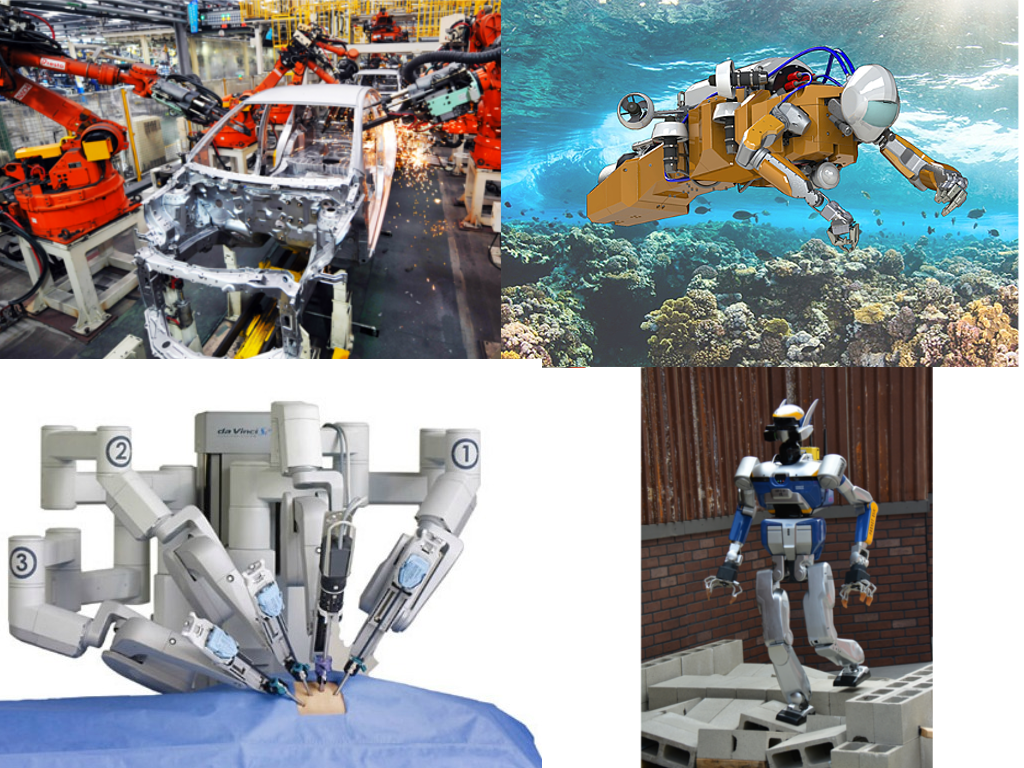
\includegraphics[width=0.9\textwidth]{various-tasks.png}
  \caption{Various robots doing various tasks}
\label{fig:various}
\end{figure}

The DARPA Robotics Challenge has brought some light on the humanoid robots.
This competition brought together a large scope of robotics groups from universities, laboratories and private companies around a common goal: teleoperate a robot to make it succeed in several challenges without any human physical intervention.
The robots were expected to drive a car, open a door, climb stairs, cross debris, drill a hole in a wall, etc.
All those tasks can usually be broken down into sets of elementary tasks in human language.
Some typical examples of tasks for a robot can be `Put hand in contact with target', `Put foot on next step', `Avoid collision with that object', `Maintain stability' or `Look in that direction'.
As is, those tasks do not mean anything for the robot.
A robot is made of a collection of bodies that are linked together by joints actuated by motors.
A robots configuration consists of the position and orientation of its base body, and the configuration of each of its joints.
Satisfying a task requires that the joints of the robot reach a configuration for which the task is satisfied.
The action of satisfying a task comes down to moving from an initial configuration to a goal.
Computing the trajectory to follow and actually following it are the jobs of the trajectory generation and the control of the robot.
Those are by themselves some complete fields of robotics, and they have one thing in common, they both need to be given an initial and a final configuration, and sometimes some intermediate ones.
Finding those configurations is the job of what we call the Posture Generator (PG).

There are two types of robots. The fixed-base robots and the mobile ones.
The first type of robots have fixed basis, the area that they can reach is predefined by their geometry and they are usually fully actuated (But not always, as they sometimes have underactuated joints).
This means that the robot has as many degrees of freedom (DoF) as actuators, Thus, for any joint configuration, a unique robots position can be achieved.
On the contrary, mobile robots are always under actuated, the robot has more DoF than actuators.
Each link of the robot is actuated, but the position of the basis of the robot depends on the configuration of the joints as a well as on the locations of the contacts that the robot makes with the environment.

%A mobile robot's position depends on the location of its contacts with the environment.
%For biped robots evolving on a flat surface, a footstep planner can be used to decide of the sequence of steps to take so the robot can walk to its goal.

Humanoid robots are expected to move and achieve tasks in ways similar to humans.
On flat surfaces, they can walk based on a cyclic motion and the locations of footsteps can be generated by a footstep planner using some simplified models to maintain the robots stability.
In cumbersome and unstructured environments, we humans move in a non-gaited acyclic way: we choose appropriate parts of our body to create contacts with the surrounding environment in order to support the motion of the remaining parts while avoiding obstacles.
A whole motion is a sequence of contact creations and releases.

Since we are biped, we mostly use our feet to move.
As the environment becomes more difficult to cross, hands may come into play together with feet to help with the motion.
Narrow passages may even require other parts of our body (knees, elbows, back\dots) to make contact in order to support the motion.

Planning the sequence of contacts to achieve is a necessary step in devising a motion for a robot.
Once the key stances of the motion have been identified by the planner, they can be used by the controller or the trajectory planner and finally the motion can be achieved by the robot.

All the aforementioned planning methods rely on the fact that we have a tool to decide if a proposed set of contact is feasible or not for the robot.
The tool used for finding a robot configuration that satisfies a set of various constraints like the geometric constraints of contact or the stability of the robot is called a `Posture Generator' (PG) and the development of that tool is the main topic of this dissertation.

The mission of a posture generator is, for a poly articulated system, to find a configuration so that the system satisfies a set of constraints.
For simple systems, with simple constraints, like a 6 DoF robotic arm having to reach a point with its end effector, some closed-form expressions can sometimes be devised.
But computing robot configuration to meet the requirements of a given set of tasks, within a viable state, is a recurrent problem whose complexity grows with that of the robot.
When the robotic problem studied becomes too complex for closed-form formulas, it is formulated as a nonlinear optimization program and solved using optimization algorithms.
The Posture Generator is a key tool of many robotics applications and as such, it is an important component of any robotics framework.
It needs to be efficient at finding a solution when one exists and at figuring when a problem is not feasible.
The speed of generating a multi-contact sequence is directly related to the quality of the posture generator, which is directly related to the quality of the optimization algorithm that it uses.

The variables of a robotics problem sometimes naturally belong to a non-Euclidean manifold $\mathcal{M}$, like $SO(3)$ for the 3D rotation of the base of a mobile robot.
A manifold is a topological space that locally resembles Euclidean space near each point.
More precisely, each point of an n-dimensional manifold has a neighbourhood that is homeomorphic to the Euclidean space of dimension n.
An n-dimensional non-Euclidean manifold cannot always be globally parameterized over a subset of $\mathbb{R}^n$ without presenting problems of singularity.
Most of the solvers available make the assumption that the search space is Euclidean and thus, do not feature the capability of solving problems on non-Euclidean manifolds natively.
But it is often possible to parametrize $\mathcal{M}$ over a higher dimensionality Euclidean space with added constraint (e.g. unit quaternions, rotation matrices).
It is then possible to solve those problems with classical solvers at the cost of additional variables, constraints and special treatments in the optimization problem.
There exists some methods and algorithms to solve optimization problems on non-Euclidean manifolds with no substantial extra cost and guaranteeing a good coverage of the manifolds without facing parameterization singularities and with the minimal number of parameters, though to our knowledge, they are focused on non-constrained optimization.

%Usually, the solver used for solving optimization problems is a black box on which the user has a very limited control.
In this thesis, we develop our own nonlinear solver on manifolds, that we use to solve optimization problems on their native search manifolds, should they be of posture generation or others.
This has the added advantage that unlike off-the-shelf solver, which are often a black box on which the user has a very limited level of control, we have full control over that solver and can specialize/modify it to fit our needs.

%\paragraph{Specificities of our approach}
%If we consider a problem of posture generation on a mobile robot with $n$ joints, the configuration space of the joints of the robot is $\mathbb{R}^n$ and the configuration space of the position and orientation of its base body is $SE(3) = \mathbb{R}^3\times SO(3)$.
%Thus, the variable that describes the configuration of the robot in the optimization problem lives in $\mathbb{R}^3\times SO(3) \times \mathbb{R}^n$.
%$SO(3)$ is by nature a non-Euclidean manifold, it cannot be parameterized on an open subset of Euclidean space without having to deal with problems of gimbal lock.
%The gimbal lock is a singularity that happens when parameterizing $SO(3)$ on $\mathbb{R}^3$, with Euler angles, for example, and when two axis of rotation become aligned, in that situation, 2 elements of the parameterization correspond to the same rotation.
%Thus, one degree of freedom is lost.
%Note that this singularity can block the optimization algorithm and that it is only due to the choice of parameterization, it is not intrinsic to the manifold $SO(3)$.
%It is possible to parameterize $SO(3)$ without having to face singularities by parameterizing it over another non-Euclidean manifold.
%The most common ones are the unit quaternion space and the $3\times 3$ rotation matrix.
%Most of the solvers available make the assumption that the search space is Euclidean, which makes is complicated to use quaternion or rotation matrix efficiently.
%To put it simply, for the unit quaternion parameterization, a variable on $SO(3)$ is represented by 4 parameters, the coefficients of the quaternion and an equality constraint needs to be added to the optimization problem to ensure that the quaternion is of norm 1, $\{q\in\mathbb{R}^4:||q||=1\}$.
%Similarly, if a variable is parameterized by a rotation matrix, then the variable $M$ has 9 parameters and several constraints need to be added to the problem so that M is symmetric, positive definite and its determinant is 1 $\{M\in\mathbb{R}^{3\times 3}:M^T M = \mathbb{I}_3\  \&\ \det (M) = 1\}$.
%Similar issues can be found with the parameterization of other non-Euclidean manifold, like $S2$ for example.

%There exists some methods and algorithms to solve optimization problems on non-Euclidean manifolds with no substantial extra cost and guaranteeing a good coverage of the manifolds without facing parameterization singularities and with the minimal number of parameters, though to our knowledge, they are focused on non-constrained optimization.

\paragraph{Contributions and plan}
The main focus of this thesis is the formulation and resolution of problems of posture generation for robotics systems using nonlinear optimization on manifolds.
Our contributions are of two types, on one hand we propose some extensions and improvements on the way to formulate a posture generation problem, and on the other hand, we investigate new ways of solving them.
The organization of this thesis is as follows:
%In Chapters~\ref{cha:state_of_the_art} and~\ref{cha:posture_generation_problem_formulation}, we present the background of posture generation, with respectively a state of the art and a presentation of the detailed formulation of a posture generation problem.
%We present several
\begin{itemize}
  \item In Chapter~\ref{cha:state_of_the_art_and_problem_definition} we give the state of the art of posture generation and optimization on manifolds.
  \item In Chapter~\ref{cha:posture_generation_problem_formulation}, we present the detailed formulation of a posture generation problem.
  \item In Chapter~\ref{cha:extensions_of_posture_generation} we present three different and unrelated contributions: two formulation extensions, one allowing to generate non-inclusive contacts between convex surfaces, the other is the exact derivation of the torques in the actuators of a robot.
  Then we present our endeavor to use the `Lifted Newton Method' to solve posture generation problems.
  \item Chapter~\ref{chapter:optimization_on_noneuclidean_manifolds} describes the principles of nonlinear optimization over non-Euclidean manifolds and our implementation of a solver based on those principles.
  \item In Chapter~\ref{ch:PG}, we present a framework that simplifies and extends the formulation of posture generation problems by formulating and solving the optimization problem over native non-Euclidean manifolds, managing automatically the variables of the problems and proposing a framework that formalizes and simplifies the writing of functions on geometric entities often used in robotics.
  \item In Chapter~\ref{cha:evaluation_and_experimentation}, we evaluate the performances of our solver on manifolds and of our posture generator. And then present a preliminary work on how to generate postures on a sensory acquired environment.
\end{itemize}


